\documentclass[dwyatte_dissertation.tex]{subfiles} 
\begin{document}

\sloppy

\chapter{The LeabraTI framework: Spatiotemporal prediction with thalamocortical rhythms}
\label{chap:leabrati}

\section{Introduction}
This chapter describes the LeabraTI (Temporal Integration) framework, which is a mechanistic description and general model of how prediction and temporal integration works in the brain. It is closely related to the Simple Recurrent Network (SRN) \cite{Elman90,Servan-SchreiberCleeremansMcClelland91} a neural network architecture that explicitly represents temporally lagged information in discrete ``context'' units whose activity gets integrated with more current information to predict what happens in the next time step (Figure \ref{fig:srn_circuit}A). This method of copying a contextual representation from an intermediate representation at discrete intervals was originally shown to be a robust way to leverage error-driven learning to represent latent temporal structure in auditory streams and artificial grammars. More generally, the SRN's explicit representation of temporally lagged context can capture the latent structure of any stimulus that varies systematically over time, making it a good basis for a generic prediction and temporal integration mechanism.

LeabraTI differs in several key ways from the classical SRN architecture, primarily in the way context is represented and used in predictive processing. These differences are due to biological constraints imposed by the microcircuitry of the neocortex, and thus form a number of testable predictions that can be used to evaluate the validity of the LeabraTI framework. The central prediction of LeabraTI is that temporally lagged context is represented by deep (Layer 6) neurons, which is possible in part to the bifurcation of intra-areal and inter-areal processing streams. As neural processing is a continuous operation, LeabraTI requires a regular interval over which to integrate deep context and make predictions, which is approximately every 100 ms. Predictions are made by driving superficial (Layers 2 and 3) neurons with the state of deep neurons through the intra-areal pathway, which is interleaved with standard peripheral sensory inputs over a total period that is also 100 ms. The strong 100 ms dependency in LeabraTI corresponds to the brain's alpha rhythm, which has been studied extensively using scalp EEG (\nopcite{MathewsonGrattonFabianiEtAl09,BuschDuboisVanRullen09,GouldRushworthNobre11,RohenkohlNobre11}; \abbrevnopcite{MathewsonPrudhommeFabianiEtAl12,BelyusarSnyderFreyEtAl13}; \nopcite{PalvaPalva07,HanslmayrGrossKlimeschEtAl11,VanRullenDubois11}). 

\textbf{TODO: Foreshadow structure of chapter...}

% srn/microcircuit fig
\begin{figure}[h!]
\begin{center}
\begin{tabular}{ll}
\textbf{A} & \textbf{B} \\
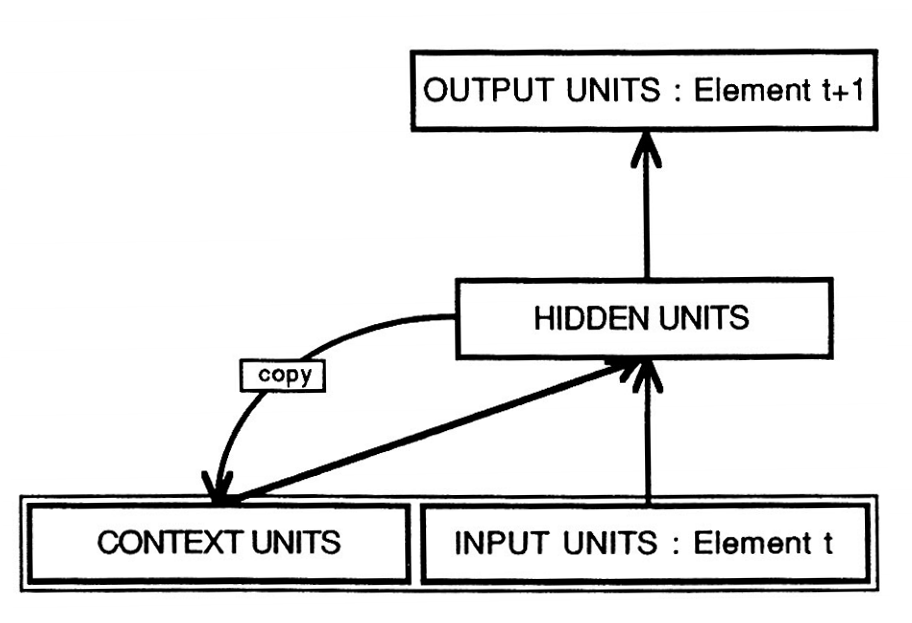
\includegraphics[width=85mm]{figs/chap_leabrati/srn_scm.png} &
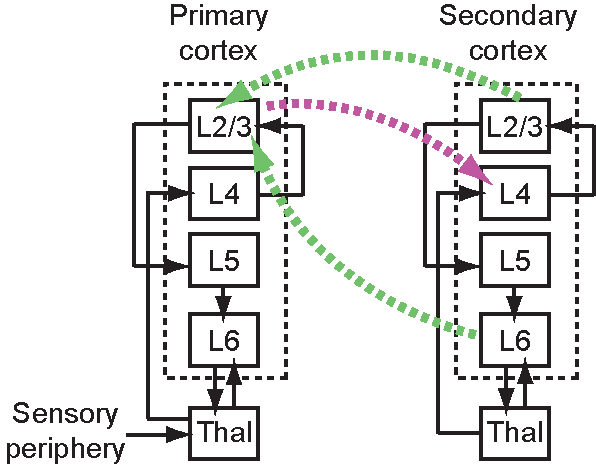
\includegraphics[width=75mm]{figs/chap_leabrati/microcircuit_horiz.pdf} \\
\end{tabular}
\end{center}
\caption{The Simple Recurrent Network (SRN) and microcircuitry of the neocortex}{\textbf{A}: The SRN represents temporal information explicitly using discrete context units that are updated once per time step. Context is integrated with more current inputs to predict information at the subsequent time step. Reproduced from \protect\incite{Servan-SchreiberCleeremansMcClelland91}. \textbf{B}: The neocortex is laminated with canonical circuitry between neurons across layers and between areas. Principal intra-areal connections are shown in black with inter-areal feedforward connections in purple and feedback connections in green.}
\label{fig:srn_circuit}
\end{figure}

\section{LeabraTI biological details}

\subsection{Laminar structure and microcircuitry of the neocortex}
A salient feature of the brain, and potential clue in realizing how an SRN-like computation might be carried out in biological neural circuits, is the laminar structure prevalent across the neocortex (Figure \ref{fig:srn_circuit}B). Incoming information from the sensory periphery is transmitted through the thalamus and targets Layer 4 neurons in the primary sensory cortices (e.g., V1). From there, Layer 4 neurons propagate spikes to superficial neurons (Layers 2 and 3) which in turn target Layer 4 neurons of higher-level cortices, forming the prominent corticocortical feedforward pathways that subserve visual and auditory recognition \cite{FellemanVanEssen91}. Corticocortical feedback originates in superficial layers or Layer 6 of the higher-level cortex and generally terminates on superficial neurons of the lower-level cortex \cite{RocklandPandya79}. In addition to these inter-areal pathways, there exists a canonical microcircuit of the form Layer 4 $\rightarrow$ Layer 2/3 $\rightarrow$ Layer 5 $\rightarrow$ Layer 6 that routes spike propagation through the local neuronal structure \cite{DouglasMartin04,ThomsonLamy07,DacostaMartin10}. This microcircuit forms the core computational unit of LeabraTI, as will be described in this and the following sections.

The importance of the local microcircuit was first suggested by Vernon Mountcastle in his proposal regarding the gross columnar organization of the neocortex \cite[see][for a comprehensive review]{Mountcastle97}. Mountcastle's proposal states that microcolumns composed of around 80-100 neurons extending vertically through all six lamina with canonical circuitry form the core repeating structure of the neocortex. Neurons within a single micrcolumnnar circuit possess nearly identical receptive field tunings across lamina while neurons in neighboring microcolumns (radial separation greater than 600 \SI{}{\micro\meter}) possess very different receptive field tunings but contribute to the higher-order macrocolumn (i.e., hypercolumn) structure \cite{HubelWiesel77,Jones00}. Microcolumns have been identified in a variety of neural systems with this electrophysiological mapping and are also prominently visible under Nissl staining. Despite this evidence for their structural existence, any function of the microcolumn aside from an organizing principle remains debated \cite{BuxhoevedenCasanova02,HortonAdams05}.

LeabraTI provides a computational role for the microcolumn, by mapping an SRN-like computation onto their Layer 4 $\rightarrow$ Layer 2/3 $\rightarrow$ Layer 5 $\rightarrow$ Layer 6 circuit (Figure \ref{fig:srn_circuit}). In this mapping, superficial neurons continuously integrate feedforward and feedback inter-areal synapses to process current information. Layer 2/3 $\rightarrow$ Layer 5 $\rightarrow$ Layer 6 provides an intra-areal pathway for explicitly representing temporal context in Layer 6 neurons, which are relatively isolated from nonlocal inputs. There is also appropriate circuitry for recirculating this context through the local microcolumn via Layer 4 to drive the learning of temporal associations. This basic idea provides a concise explanation for the strong degree of isotuning throughout a single microcolumn, as Layer 6 neurons need to represent the same overall information as superficial neurons except at a delayed interval.

\subsection{Layer 5 rhythmic bursting and contextual gating}
The laminocolumnar organization of the neocortex provides the dual pathways necessary for continuous information processing and the SRN's explicit temporal context representation. The Layer 4 $\rightarrow$ Layer 2/3 $\rightarrow$ Layer 5 $\rightarrow$ Layer 6 microcircuit only contains four synapses plus the transthalamic re-entrant synapses. Intracolumnar monosynaptic latencies for regular spiking neurons are on the order of 5 ms or faster \cite{Armstrong-JamesFoxDas-Gupta92,LumerEdelmanTononi97} and thus this relatively small amount of tissue, if driven with constant input, would circulate spikes at a rate too fast to perform enough temporal integration to make useful predictions. Several studies have noted that a subset of Layer 5 neurons exhibit intrinsic bursting at $\sim$10 Hz when over threshold (\nopcite{ConnorsGutnickPrince82,SilvaAmitaiConnors91}; \abbrevnopcite{FranceschettiGuatteoPanzicaEtAl95}). This rhythmic busting might implement a gating mechanism for updating Layer 6 context information at a regular 100 ms interval.

More specifically, Layer 5 neurons can be roughly divided into 5a and 5b subtypes \cite{ThomsonLamy07}. Layer 5a neurons have relatively small cell bodies and exhibit regular spiking depolarization responses. They collect input from other Layer 5a neurons both within and across columns \cite{SchubertKotterStaiger07} and pass it to 5b neurons and thus, likely play a simple information integration role. Layer 5b neurons, in contrast, have larger cell bodies and exhibit the aforementioned 10 Hz intrinsic bursting response profile. In the context of LeabraTI, the interpretation of this data is that the 5a neurons serve to integrate information from multiple Layer 2/3 neurons, with the 5b neurons gating context to Layer 6 neurons with each 10 Hz burst.

Layer 6 corticothalamic neurons receive strong inputs from Layer 5b neurons and send axons toward the thalamus completing the microcircuit within the local column and allowing the temporally lagged Layer 6 responses to integrate with more current Layer 4 inputs. Information is relayed from the thalamus back up to layer 4 in a focal one-to-one manner that maintains microcolumnar separation \cite{ShermanGuillery06,Thomson10}, which could allow temporal associations to be formed by local Hebbian learning mechanisms that track high probability co-occurences across past and present events \cite{Foldiak91}.

\subsection{Thalamic gating and sensory prediction}
Both the SRN computation and the Leabra algorithm \cite{OReillyMunakata00,OReillyMunakataFrankEtAl12} that are used to implement the LeabraTI framework are predicated on using powerful error-driven learning mechanisms (in addition to more standard Hebbian learning mechanisms) to represent the mapping between sensory inputs and outputs. In the context of temporal integration, error-driven learning would allow computation of error signals based on the difference between what is predicted to happen at a given moment (given the previous moments context as an input) and what actually happens. However, this computation requires that both the prediction and the actual sensation are represented by the same neural tissue so that an error signal can be computed, which is not possible if the sensory periphery is continuously transmitting incoming inputs. 

To resolve this issue, the LeabraTI framework posits that predictions about sensory events and the sensory events themselves are temporally interleaved through the same population of neurons in an alternating manner. This requires a mechanism to periodically downmodulate or even block the transmission of inputs from the sensory periphery. A subset of cells in the thalamus exhibit $\sim$10 Hz intrinsic bursting properties similar to that of Layer 5 neurons (\nopcite{LopesdaSilva91}; \abbrevnopcite{HughesLorinczCopeEtAl04}; \nopcite{LorinczCrunelliHughes08}; \nopcite{LorinczKekesiJuhaszEtAl09}), and thus perhaps perform a similar gating computation of sensory inputs into cortical circuits. In the context of LeabraTI, these bursting neurons might shift the balance of inputs to Layer 4 and superficial neurons between endogenous inputs local to the microcolumn representing predictions and quick bursts of actual sensory information. 

More specifically, during the non-bursting intervals of thalamic intrinsically bursting neurons' response, environmental inputs are downmodulated due to the relative quiescence and Layer 6 neurons provide the dominant driving potential to the microcolumn. Layer 6 corticothalamic neurons exhibit a strong regular spiking depolarization response with facilitating short-term dynamics \cite{Thomson10} unlike all other pyramidal neurons, which exhibit depressing dynamics. This might suggest a specialized function for Layer 6 neurons, which in the context of LeabraTI is to drive a sustained prediction about upcoming sensory information. These layer corticothalamic neurons also sustain their drive through reciprocal projections with the thalamic relay cells that they project to. In addition to the Layer 6 $\rightarrow$ Layer 4 transthalamic pathway, Layer 6 neurons also project directly to Layer 4. While these projections are relatively weak \cite{HirschMartinez06b}, they do activate a metabotropic glutamate receptor (mGluR) that produces sustained depolarization similar to Layer 6 corticothalamic neurons \cite{LeeSherman09} -� these direct ascending synapses are another possible route for sustained context information to drive Layer 4 neurons. 

The burst response of thalamic intrinsic bursting neurons synchronized with the burst response of Layer 5b neurons destabilizes the Layer 6 sustained prediction through biased competition. This provides a snapshot of the current state of the sensory periphery as well as an opportunity to integrate the state of current sensory event into a prediction about what will happen during the next moment. At this time, standard error-driven learning mechanisms that compute short timescale firing rate differences \cite{OReillyMunakata00,OReillyMunakataFrankEtAl12} compute an error signal between the previous moment's prediction and the sensory outcome to minimize overall prediction error.

\section{Summary of LeabraTI computation}
The overall computation of LeabraTI is shown in Figure \ref{fig:leabrati_comp} and summarized here. Standard Leabra processing operates across two phases: a \textit{minus} phase that represents the system's expectation for a given input and a \textit{plus} phase, representing observation of the outcome. Generally, feedforward sensory inputs provide the dominant drive during the minus phase while the plus phase is driven by a combination of feedforward sensory inputs and the target outcome, conveyed via feedback projections. Leabra networks typically only model at the level of superficial (Layers 2 and 3) neurons, since they provide the principal feedforward and feedback projections necessary for error-driven learning.

% leabrati computation
\begin{figure}[h!]
\begin{center}
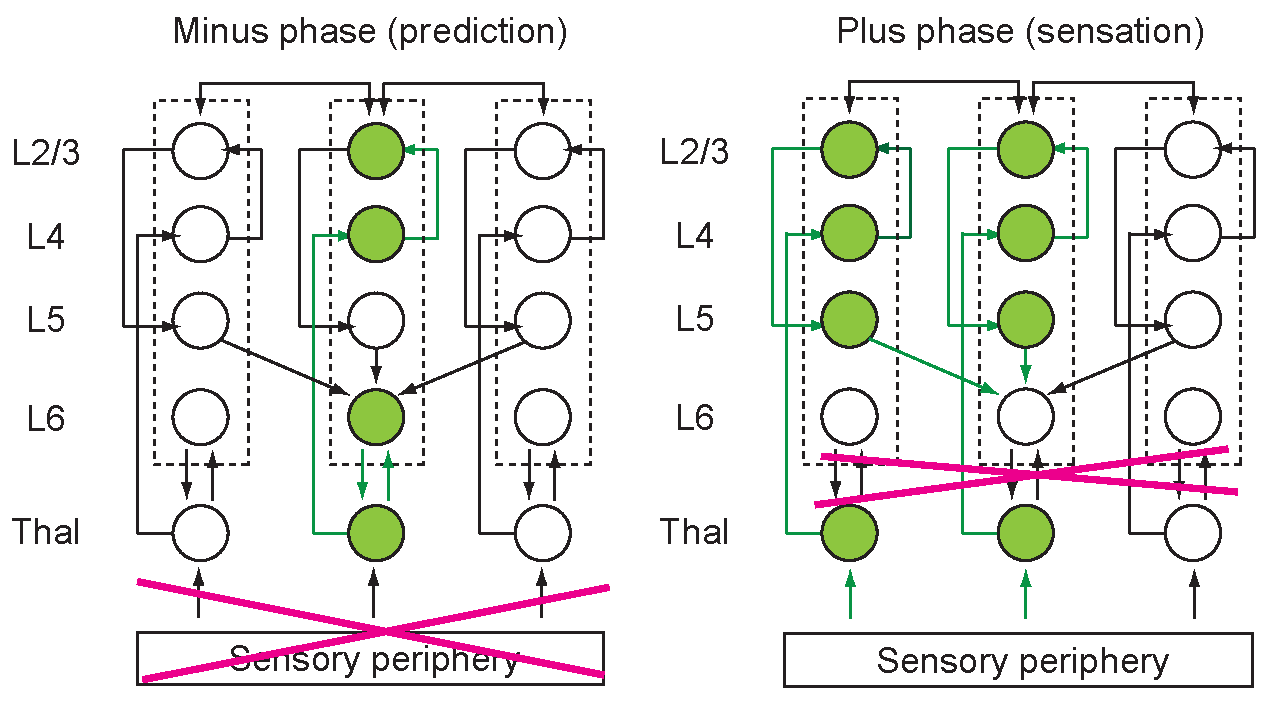
\includegraphics[width=160mm]{figs/chap_leabrati/leabrati_comp_new.pdf}
\end{center}
\caption{The LeabraTI computation}{LeabraTI consists of a \textit{minus} phase prediction about what is about to happen in the following \textit{plus} phase sensory event. The minus phase is characterized by a sustained prediction from deep Layer 6 neurons based on lagged context from the previous moment. Input from the sensory periphery is extremely downmodulated or even blocked during the minus phase due to the relative quiescence of thalamic intrinsically bursting neurons. The plus phase is characterized by a rapid burst of information from the sensory periphery that drives also drives Layer 5 intrinsically bursting neurons to threshold so that they can integrate a snapshot of the current moment as context. Full feedforward and feedback-mediated processing is active in both phases so that predictions are not entirely dependent on deep Layer 6 neurons, but can also be driven by higher-level expectations.}
\label{fig:leabrati_comp}
\end{figure}

In LeabraTI, deep Layer 6 neurons provide the dominant input to superficial Layer 2/3 neurons during the minus phase, relayed via Layer 4 transthalamic and direct ascending projections (not pictured in Figure \ref{fig:leabrati_comp}). This represents a sensory prediction about what is about to happen during the subsequent plus phase, using temporally lagged context from the previous plus phase. To be computationally useful, the prediction needs to last at least 50 ms in order to allow contributions from both the feedforward drive and slightly longer latency feedback from higher-order cortical areas. The short-term facilitating dynamics unique to Layer 6 corticothalamic neurons or mGluR activation from the direct ascending projections provide the sustained spiking response throughout the minus phase. Reciprocal thalamocortical synapses back to Layer 6 might also assist in maintaining minus phase input drive. During this period, input from the sensory periphery is extremely downmodulated due to the relative quiescence of thalamic intrinsically bursting neurons. Downstream areas basically repeat this predictive process driven by their respective deep Layer 6 context, although they do also receive direct Layer 4 drive from the previous cortical area. 

The plus phase is characterized by a shift of input from the local column to the sensory periphery, driven by the destabilizing response from thalamic intrinsically bursting cells. The rapid influx of synchronous drive from the thalamus serves two purposes. First, it rapidly drives the propagation of responses through downstream areas by quickly driving neurons along the feedforward Layer 4 $\rightarrow$ Layer 2/3 $\rightarrow$ Layer 4 pathway \cite{FellemanVanEssen91} to threshold, similar to the concept of ``synfire chains'' that simultaneously ignite entire pools of neurons to propagate waves of spikes back and forth through a network \cite{BrunoSakmann06,WangSpencerFellousEtAl10,TiesingaFellousSejnowski08}. Second, it drives responses down through the Layer 2/3 $\rightarrow$ Layer 5 $\rightarrow$ Layer 6 pathway, which also requires a large influx of thalamic drive \cite{BeierleinFallRinzelEtAl02}. This rapid transmission between and within areas causes Layer 5b neurons across areas to burst with relatively little cross-area delay so that the context that the bursting captures represents information from a single moment in time.

Once thalamic bursting quiets, the input to the microcolumn shifts back to the newly integrated Layer 6 context. This prediction-sensation process repeats approximately every 100 ms corresponding to the brain's alpha rhythm, which is suggested to have strong thalamocortical and deep laminar sources \cite{LopesdaSilva91,KlimeschSausengHanslmayr07,PalvaPalva07,LorinczKekesiJuhaszEtAl09,HanslmayrGrossKlimeschEtAl11,BuffaloFriesLandmanEtAl11}. 

\section{Relation to other frameworks}

\subsection{The Simple Recurrent Network (SRN)}
LeabraTI is perhaps most closely related to the Simple Recurrent Network (SRN) \cite{Elman90,Servan-SchreiberCleeremansMcClelland91}, but with several key differences that are necessary due to the implementation using cortical circuits. The SRN is capable of learning temporal sequences by virtue of a ``copy'' operation (Figure \ref{fig:srn_invert}) that represents an exact replica of the previous time step's intermediate units in separate group of context units. Thus, the SRN integrates two inputs at each time step -- the previous time step's processed inputs and the current time step's unprocessed inputs. Predictions are made in a separate group of output units and prediction errors are backpropagated to learn the weights that allow the best prediction over items in the input sequence. 

Like the SRN, LeabraTI uses discrete context units (deep Layer 6 neurons), but it does not implement a direct copy of sending units at each time step that is then used for predictive learning. LeabraTI is actually an inversion of the SRN formulation, where context is immediately sent through plastic integrative synapses and then through an additional input channel when computing the activation states of superficial (Layer 2 and 3) units (Figure \ref{fig:srn_invert}). The LeabraTI formulation is mathematically equivalent to the SRN, and provides a better fit with the circuitry of the microcolumn, which contains plastic synapses between Layer 5 and Layer 6 (primarily the 5a $\rightarrow$ 5b integrative synapses). The inversion also allows a sustained, uncorrupted minus phase prediction that would not be possible if the directionality of the projections were reversed due to the massive numbers of afferent and efferent synapses on superficial neurons. 

% srn/microcircuit fig
\begin{figure}[h!]
\begin{center}
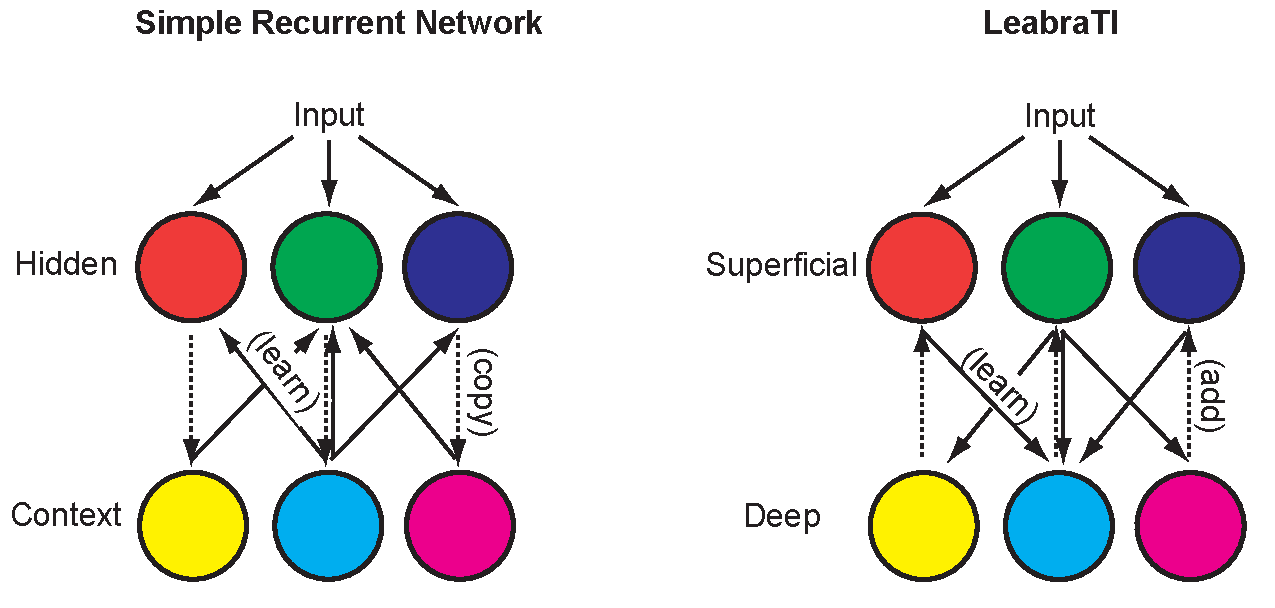
\includegraphics[width=140mm]{figs/chap_leabrati/srn_invert.pdf}
\end{center}
\caption{Relationship between the Simple Recurrent Network (SRN) and LeabraTI}{The Simple Recurrent Network (SRN) projects a direct copy of Hidden units' state to context units that is then integrated at the next time step with the current input. LeabraTI, in contrast, projects first through Layer 5 $\rightarrow$ Layer 6 plastic synapses triggering an immediate prediction that is then used additively in computing the input at the next time step. These operations are mathematically equivalent, but LeabraTI provides a better fit with the circuitry of the microcolumn.}
\label{fig:srn_invert}
\end{figure}

One other difference between LeabraTI and the SRN is that the latter makes predictions using a separate group of output units. LeabraTI, in contrast, makes predictions using the same neural tissue that is used to represent sensory outcomes. This is a much more natural mechanism for predictive learning as it does not require a separate populations of neurons for predictions and sensations -- it does, however, tradeoff the neural space savings with temporal interleaving of predictions and sensory outcomes, which could cause discretization artifacts and other temporal oddities in perception. There is increasing evidence of discretization at the $\sim$10 Hz rate proposed by LeabraTI \cite{VanRullenReddyKoch05,VanRullenReddyKoch06,AmanoArnoldTakedaEtAl08,BuschDuboisVanRullen09,SokoliukVanRullen13,VanRullenKoch03b,VanRullenDubois11}, which is discussed in the section following this one. 

% columns are essentially bio SRN's, shifts computational unit from neuron to microcolumn

\subsection{Predictive coding models}
Another framework related to LeabraTI is the predictive coding model \cite{RaoBallard99,Friston05,DenOudenKokDeLange12}. The fundamental claim of predictive coding models is that sensory events themselves are not explicitly encoded by neurons. Instead, prediction errors -- the difference between predictions and sensory events -- are what is encoded. The prediction error computation is generally repeated at each stage of processing with only the residual error being propagated downstream for further processing. Predictive coding models have gained traction due to this efficient ``delta'' code and due to their positing a distinct role for feedback projections in generating predictions. A recent description of predictive coding makes contact with the microcolumnar circuitry in the same way as LeabraTI. In their proposal, \abbrevincite{BastosUsreyAdamsEtAl12} suggested that deep infragranular neurons code prediction errors which ascend back to Layer 4 neurons or down to lower-level areas as feedback predictions. 

The primary problem with predictive coding models is in their computation of prediction error. This computation requires feedback predictions to be inhibitory in nature so that they can be subtracted from the excitatory input, leaving only the residual error. This computation is not possible in cortical circuits since feedback via pyramidal axons is fundamentally excitatory. This issue could be resolved by inverting the excitatory signal, but feedback axons predominantly target other excitatory cells and the net postsynaptic potentials generated by their activation are also excitatory \cite{Budd98,JohnsonBurkhalter96,JohnsonBurkhalter97}.

LeabraTI resolves this issue by computing predictions and sensory events explicitly in discrete phases, based on excitatory input with inhibitory competition to suppress spurious errors in coding \cite{WyatteHerdMingusEtAl12,DesimoneDuncan95}. Thus predictions are not fundamentally inhibitory, but excitatory due to being driven through Layer 4 neurons from deep context. This assumption is consistent with predictive remapping \cite{DuhamelColbyGoldberg92,NakamuraColby02,CavanaughHuntAfrazEtAl10} in cortex during which excitatory neurons fire in anticipation of a stimulus that is outside of their receptive field but will be entered upon making a saccade.

% To generate reasonable expectations, it is essential to sustain and integrate information from the past
\section{LeabraTI testable predictions}
%More generally, LeabraTI's dichotomy of continuous integration in superficial layers and periodic updating of deep layers receives strong support by the literature. Recent studies that have employed depth electrodes to simultaneously record from multiple layers within a patch of cortex have indicated that superficial layers exhibit spectral power at much higher frequencies than deep layers. \incite{BuffaloFriesLandmanEtAl11} recorded responses from ventral visual sites V1, V2, and V4 in awake, behaving monkeys during a simple directed attention task, finding a dissociation in spike coherence frequency in superficial (gamma spectrum, peak $\sim$50 Hz) and deep layers (alpha spectrum, peak $\sim$10 Hz). A similar experimental paradigm expands on these findings by demonstrating cross-frequency coupling between gamma and alpha spectra localized to superficial and deep layers, respectively \cite{SpaakBonnefondMaierEtAl12}. % say something about modulation here
%The cross-frequency coupling is characterized by a clear nesting of gamma activity within alpha cycles, suggesting that deep neurons' alpha activity might subserve a general pacemaker mechanism. In the context of LeabraTI, this pacemaker property is important to ensure the regular updating of context through deep layers and temporally predictable reintegration with more current information.
% Spaak: within the lower frequency alpha oscillations and an inverse relationship in which alpha attenuation resulted in higher amplitude and longer lasting gamma activity (and vice versa)

%This rhythmic firing has been shown to persist even with constant sensory stimulation \textit{in vivo} \cite{LuczakBarthoHarris13}, suggesting that Layer 5 neurons' alpha rhythmicity could implement a roughly 10 Hz gating function for spikes relayed to Layer 6 neurons. % get rid of gating, change to updates/periodicities
% need to talk about two types of layer 6 neurons and how one of them integrates broader context of L5 bursts -- make sure this is compatible with biology i.e., multiple L5b guys project to 1 of the broad RF L6 guys

% Importantly, during both the prediction and sensation phases, feedforward and feedback projections are constantly transmitting between lower and higher cortical areas. As previously mentioned, these projections originate and terminate predominantly in superficial layers, boosting their spike coherence to higher frequency spectra. This could potentially explain the differentially high gamma power in superficial layers compared to deep layers, and provides a compelling link between gamma oscillations and predicting specific details about the next sensory event.

%Thus, Layer 6 specifically becomes the neural substrate of the SRN's temporally lagged context representation, representing information that is, on average, one alpha cycle (approximately 100 ms) in the past. This contextual storage occurs at an automatic interval due to the intrinsic pacemaking properties of Layer 5 neurons, and might implement a reference frame that essentially would allow the brain to know \textit{when} to anticipate inputs. As such, intrinsic oscillations have been shown to phase lock to environmental stimulation \cite{WillBerg07,LakatosKarmosMehtaEtAl08,SchroederLakatos09,StefanicsHangyaHernadiEtAl10}, ensuring environmental events coincide with key events like Layer 5 bursts in cortex. % need to unpack this entrainment idea and motivate prediction without corruption

% short bit about general predictions regarding synchronicity between layers, latencies and how readout should be 100 ms in past, etc.
% but focus of this section will be on EEG predictions
% * Alpha entrainment, classic alpha effects -- see RFI for topics to hit
% * 	Nobre, Busch, VanRullen, Mathewson, etc.
% * 	prediction/sensation interleaving, basic evidence for this, to be tested further with my experiments
% *		Role of attention vs. prediction


%\bibliographystyle{apa}
%\bibliography{ccnlab}

% OTHER TODO
% * Nesting of gamma within alpha, and actually is the ``duty cycle'' -- need to reread Spaak, Jensen papers
% * analogies about carrier signals/duty cycles?

\end{document}